% !TeX spellcheck = en_US
\documentclass[12pt]{article}

\usepackage{fancyhdr} % Required for custom headers
\usepackage{lastpage} % Required to determine the last page for the footer
\usepackage{extramarks} % Required for headers and footers
\usepackage[usenames,dvipsnames]{color} % Required for custom colors
\usepackage{graphicx} % Required to insert images
\usepackage{listings} % Required for insertion of code
\usepackage{courier} % Required for the courier font
\usepackage{lipsum} % Used for inserting dummy 'Lorem ipsum' text into the template
\usepackage{amsmath}
\usepackage{caption}
\usepackage{multirow}
\usepackage{graphicx}
\usepackage{amssymb}
\usepackage{caption}
\usepackage{subcaption}
\usepackage{algorithm}
\usepackage{algpseudocode}
\usepackage{epstopdf}
\usepackage[dvipsnames]{xcolor}
% Margins
\topmargin=-0.45in
\evensidemargin=0in
\oddsidemargin=0in
\textwidth=6.5in
\textheight=9.0in
\headsep=0.25in
\headheight=15.0pt


\linespread{1.1} % Line spacing

% Set up the header and footer
\pagestyle{fancy}
\lhead{\hmwkAuthorName} % Top left header
\chead{\hmwkClass: \hmwkTitle} % Top center head
\cfoot{} % Bottom center footer
\rfoot{Page\ \thepage\ of\ \protect\pageref{LastPage}} % Bottom right footer
\renewcommand\headrulewidth{0.4pt} % Size of the header rule
\renewcommand\footrulewidth{0.4pt} % Size of the footer rule

\setlength\parindent{0pt} % Removes all indentation from paragraphs

%----------------------------------------------------------------------------------------
%	DOCUMENT STRUCTURE COMMANDS
%	Skip this unless you know what you're doing
%----------------------------------------------------------------------------------------

% Header and footer for when a page split occurs within a problem environment
\newcommand{\enterProblemHeader}[1]{
	\nobreak\extramarks{#1}{#1 continued on next page\ldots}\nobreak
	\nobreak\extramarks{#1 (continued)}{#1 continued on next page\ldots}\nobreak
}

% Header and footer for when a page split occurs between problem environments
\newcommand{\exitProblemHeader}[1]{
	\nobreak\extramarks{#1 (continued)}{#1 continued on next page\ldots}\nobreak
	\nobreak\extramarks{#1}{}\nobreak
}

\setcounter{secnumdepth}{0} % Removes default section numbers
\newcounter{homeworkProblemCounter} % Creates a counter to keep track of the number of problems

\newcommand{\homeworkProblemName}{}
\newenvironment{homeworkProblem}[1][Problem \arabic{homeworkProblemCounter}]{ % Makes a new environment called homeworkProblem which takes 1 argument (custom name) but the default is "Problem #"
	\stepcounter{homeworkProblemCounter} % Increase counter for number of problems
	\renewcommand{\homeworkProblemName}{#1} % Assign \homeworkProblemName the name of the problem
	\section{\homeworkProblemName} % Make a section in the document with the custom problem count
	\enterProblemHeader{\homeworkProblemName} % Header and footer within the environment
}{
	\exitProblemHeader{\homeworkProblemName} % Header and footer after the environment
}

\newcommand{\problemAnswer}[1]{ % Defines the problem answer command with the content as the only argument
	\noindent\framebox[\columnwidth][c]{\begin{minipage}{0.98\columnwidth}#1\end{minipage}} % Makes the box around the problem answer and puts the content inside
}

\newcommand{\homeworkSectionName}{}
\newenvironment{homeworkSection}[1]{ % New environment for sections within homework problems, takes 1 argument - the name of the section
	\renewcommand{\homeworkSectionName}{#1} % Assign \homeworkSectionName to the name of the section from the environment argument
	\subsection{\homeworkSectionName} % Make a subsection with the custom name of the subsection
	\enterProblemHeader{\homeworkProblemName\ [\homeworkSectionName]} % Header and footer within the environment
}{
	\enterProblemHeader{\homeworkProblemName} % Header and footer after the environment
}

%----------------------------------------------------------------------------------------
%	NAME AND CLASS SECTION
%----------------------------------------------------------------------------------------

\newcommand{\hmwkTitle}{Assignment\ \#4} % Assignment title
\newcommand{\hmwkClass}{Advanced Image Processing} % Course/class
\newcommand{\hmwkClassInstructor}{Jones} % Teacher/lecturer
\newcommand{\hmwkAuthorName}{Shikhar Vashishth} % Your name
\newcommand{\hmwkAuthorID}{M.Tech CSA - 13374} % Your ID

%----------------------------------------------------------------------------------------
%	TITLE PAGE
%----------------------------------------------------------------------------------------

\title{
	\vspace{2in}
	\textmd{\textbf{\hmwkClass}}\\ 
	\textmd{\textbf{\hmwkTitle}}\\
	\vspace{3in}
}

\author{\textbf{\hmwkAuthorName} \\ {\small \hmwkAuthorID}}
\date{} % Insert date here if you want it to appear below your name

%----------------------------------------------------------------------------------------

\begin{document}
	
	\maketitle
	\newpage
	
	\begin{homeworkProblem}
	\subsection{Part (a): Segmentation with a simple image}
	I chose the following simple image and its synthetic version for clustering. 
	\begin{figure}[h]
		\centering
		\begin{subfigure}[b]{0.47\textwidth}
			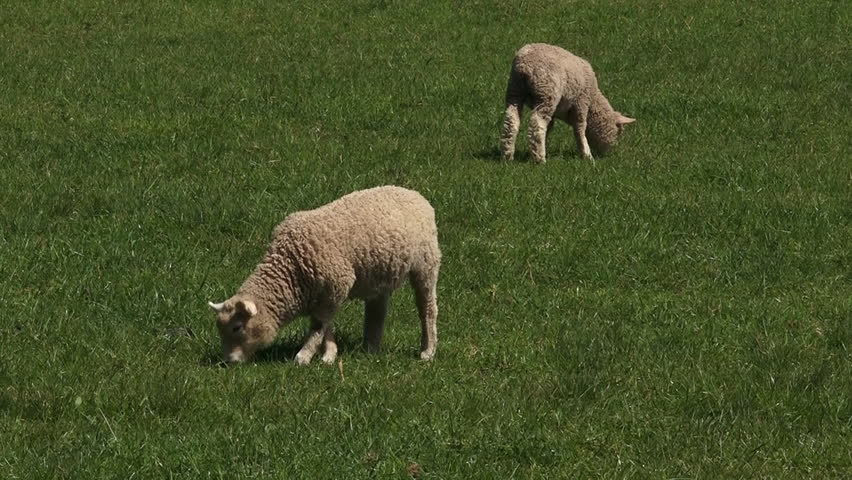
\includegraphics[width=\textwidth]{../Images/input.jpg}
			\caption{Simple Image}
		\end{subfigure}
		\hfill
		\begin{subfigure}[b]{0.47\textwidth}
			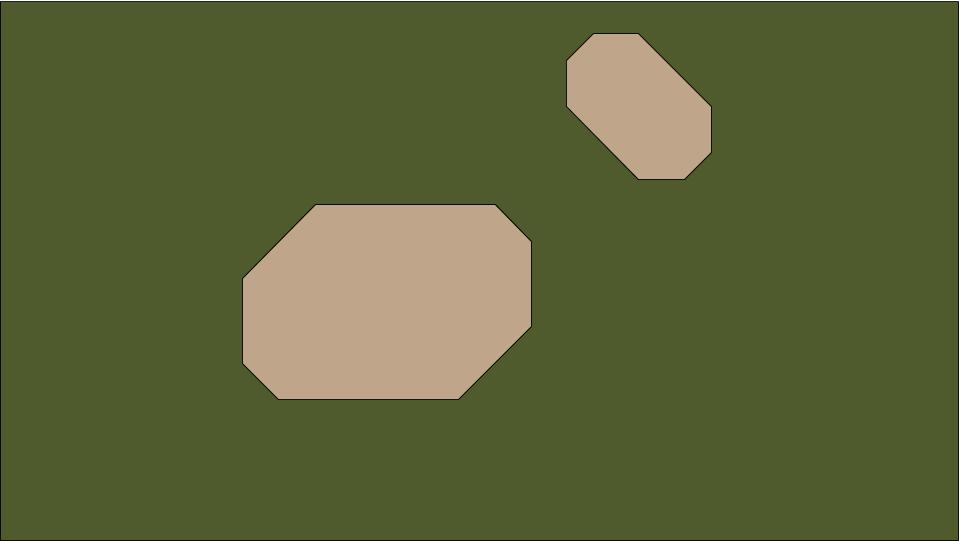
\includegraphics[width=\textwidth]{../Images/input_simple.jpg}
			\caption{Synthetic Image}
		\end{subfigure}
		\caption{Images for clustering}
	\end{figure}

	
	\begin{figure}[!htb]
		\centering
		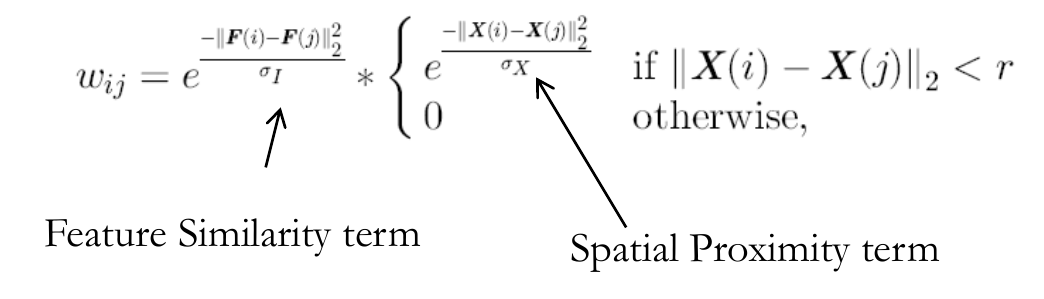
\includegraphics[width=10.5cm]{../Images/params.png}
	\end{figure}
	\textbf{Parameters}: $\sigma_I$, $\sigma_X$, $r$, ($thresh$) threshold for the 2nd eigen vector.
	
	\subsubsection{Results}
	Before applying N-cut algorithm, I first down-sampled the original image for reducing the computation. I have tried segmenting image with and without using spatial information. From the results below, we can see that although there is not much difference in the case of synthetic image but with the original image the segmentation results are better if we use the spatial information. Instead of directly using RGB values, I have used HSV values and have defined feature vector as:
	$$F(i) = [v,v.s.\sin{h}, v.s.\cos{h}] $$
	\textbf{Parameters used}: $\sigma_I = 5, \sigma_X = 5, r = 0.5, thresh = 0$\\
	
	In the figure below, the first column shows the down-sampled version of the original image used for segmentation. The other two columns show the two segments obtained from the algorithm. Overall, for both the images the results are quite satisfactory. \\
	
	
	\newpage
	\textbf{Without using spatial information}
	\begin{figure}[!htb]
		\centering
		\includegraphics[width=15.5cm]{../Output/a1_wo1.jpg}
	\end{figure}

	\begin{figure}[!htb]
		\centering
		\includegraphics[width=15.5cm]{../Output/a2_wo.jpg}
	\end{figure}
	
	\textbf{Using spatial information}
	\begin{figure}[!htb]
		\centering
		\includegraphics[width=15.5cm]{../Output/a1_w.jpg}
	\end{figure}

	\begin{figure}[!htb]
		\centering
		\includegraphics[width=15.5cm]{../Output/a2_w.jpg}
	\end{figure}
	
	\paragraph{Observations}
	In the above cases, I have used the same value of $\sigma$ for both feature and spatial similarity, but instead if we use a smaller value of $\sigma_I$ that would imply giving more emphasis to feature similarity compared to spatial similarity. The following results shows that how that would affect our segmentation results. We can see that some part of animal got segmented in the wrong segment. 
	\begin{figure}[!htb]
		\centering
		\includegraphics[width=15.5cm]{../Output/a1_o1.jpg}
		\caption{Segmentation with emphasis on feature similarity}
	\end{figure}
	
	\newpage
	\subsection{Part (b): Segmentation with a difficult image}
	I have used the following  image for evaluating N-cut algorithm with different parameters:

	\begin{figure}[!htb]
		\centering
		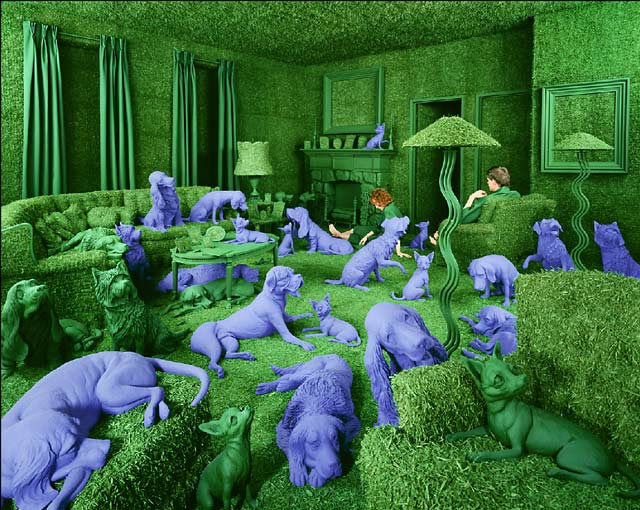
\includegraphics[width=8.5cm]{../Images/green_house.jpg}
		\caption{Complex image for segmentation}
	\end{figure}

	
	\subsubsection{Observations}
	\begin{enumerate}
		\item The spatial information is a must for complex images. In the previous part, we got decent results even without using spatial information of the pixels, but in the complex image ignoring spatial information gives unacceptable results. 
		
		\begin{figure}[!htb]
			\centering
			\includegraphics[width=13cm]{../Output/b1_o1.jpg}
			\caption{Results with $\sigma_I = 0.5$ and $\sigma_X = \infty$}
		\end{figure}
	
		We can see from the above results that because of ignoring spatial information we got discontinuity in the computed segments.
		
		\item \textbf{Keeping $\sigma_I$ very large and trying different values of $\sigma_X$.}
		
 		Small value of $\sigma_X$ implies that we are giving more weightage to the spatial similarity between pixels than feature similarity between them. 
 		
 		\begin{figure}[!htb]
 			\centering
 			\includegraphics[width=13cm]{../Output/b1_o2.jpg}
 			\caption{Results with $\sigma_I = 15$ and $\sigma_X = 0.1$}
 		\end{figure}
 		
		\begin{figure}[!htb]
			\centering
			\includegraphics[width=13cm]{../Output/b1_o2_1.jpg}
			\caption{Results with $\sigma_I = 15$ and $\sigma_X = 1$}
		\end{figure}
		
		\begin{figure}[!htb]
			\centering
			\includegraphics[width=13cm]{../Output/b1_o2_2.jpg}
			\caption{Results with $\sigma_I = 15$ and $\sigma_X = 2$}
		\end{figure}
	
		\begin{figure}[!htb]
			\centering
			\includegraphics[width=13cm]{../Output/b1_o2_10.jpg}
			\caption{Results with $\sigma_I = 15$ and $\sigma_X = 10$}
		\end{figure}
	
		\begin{figure}[!htb]
			\centering
			\includegraphics[width=13cm]{../Output/b1_o2_15.jpg}
			\caption{Results with $\sigma_I = 15$ and $\sigma_X = 15$}
		\end{figure}
		
		The above results shows us that as we increase the value of $\sigma_X$ the clusters obtained will be better, or in other words, lesser importance to spatial similarity than feature similarity improves the quality of results.
		
		\newpage
		\item In the above experimentation, I also found out that while segmenting the image based on the second eigen vector, it is better to use the mean of the values of eigen vector rather than using $0$ always. The following plot fortifies this observation. We can clearly see that the values of eigen vector are not symmetrically distributed around $0$. 
		
		\begin{figure}[!htb]
			\centering
			\includegraphics[width=12cm]{../Output/plot_eigen_vec.png}
			\caption{Distribution of values of 2nd eigen vector}
		\end{figure}
		
		The visual results also supports this observation. We can see that using mean gave us better segments as compared to using $0$. 
		\begin{figure}[!htb]
			\centering
			\includegraphics[width=13cm]{../Output/b1_o3_2.jpg}
			\caption{Segmenting eigen vector around 0}
		\end{figure}
	
		\begin{figure}[!htb]
			\centering
			\includegraphics[width=13cm]{../Output/b1_o3_1.jpg}
			\caption{Segmenting eigen vector using the mean of its values}
		\end{figure}
		\newpage
		\item Keeping $\sigma_X$ fixed at 1, I have compared the results of N-cut algorithm for different values of $\sigma_I$:
		
		\begin{figure}[!htb]
			\centering
			\includegraphics[width=13cm]{../Output/b1_o4_1.jpg}
			\caption{Results with $\sigma_I = 1$ and $\sigma_X = 1$}
		\end{figure}
	
		\begin{figure}[!htb]
			\centering
			\includegraphics[width=13cm]{../Output/b1_o4_2.jpg}
			\caption{Results with $\sigma_I = 2$ and $\sigma_X = 1$}
		\end{figure}
	
		\begin{figure}[!htb]
			\centering
			\includegraphics[width=13cm]{../Output/b1_o4_5.jpg}
			\caption{Results with $\sigma_I = 5$ and $\sigma_X = 1$}
		\end{figure}
		
		\begin{figure}[!htb]
			\centering
			\includegraphics[width=13cm]{../Output/b1_o4_10.jpg}
			\caption{Results with $\sigma_I = 10$ and $\sigma_X = 1$}
		\end{figure}
		
		\begin{figure}[!htb]
			\centering
			\includegraphics[width=13cm]{../Output/b1_o4_15.jpg}
			\caption{Results with $\sigma_I = 15$ and $\sigma_X = 1$}
		\end{figure}
		
		 From all the observation, with $\sigma_I = 5$ and $\sigma_X = 1$ the segmentation results are the best as the blue dogs got completely separated by this choice. The green dogs can be segmented by again applying N-cut to the first segment.
	\end{enumerate}
	
	\newpage
	\subsection{Part (c): Applying 2-cuts more than once}
	For this part, I am using the same image which was used in the previous part. After applying 2-cut on the original image the results are the following:
	
	\begin{figure}[!htb]
		\centering
		\includegraphics[width=13cm]{../Output/c1_s1.jpg}
		\caption{Results after first segmentation}
	\end{figure}
	
	\subsubsection{Results after second segmentation with different parameters:}
	\begin{figure}[!htb]
		\centering
		\includegraphics[width=13cm]{../Output/c1_20_30.jpg}
		\caption{Results with $\sigma_I = 20$ and $\sigma_X = 30$ (Best result)}
	\end{figure}

	\begin{figure}[!htb]
		\centering
		\includegraphics[width=13cm]{../Output/c1_10_1.jpg}
		\caption{Results with $\sigma_I = 10$ and $\sigma_X = 1$}
	\end{figure}
	
	\begin{figure}[!htb]
		\centering
		\includegraphics[width=13cm]{../Output/c1_50_100.jpg}
		\caption{Results with $\sigma_I = 50$ and $\sigma_X = 100$}
	\end{figure}

	\begin{figure}[!htb]
		\centering
		\includegraphics[width=13cm]{../Output/c1_50_25.jpg}
		\caption{Results with $\sigma_I = 50$ and $\sigma_X = 25$}
	\end{figure}

\newpage
\subsubsection{Observations:}
\begin{enumerate}
	\item On applying 2-cut again to the first segment, I got the following results with different parameters. Among all of them $\sigma_I = 20$ and $\sigma_X = 30$ gave me the best results. As can be seen in the figure, we successfully segmented out green dogs from the image which are very difficult to segment out even by a human being in such a low resolution image.

	\item The above results shows that too small value of $\sigma_X$ compared to $\sigma_I$ is a poor choice. Taking equal value for both of these parameters and taking $\sigma_I$ to be smaller than $\sigma_X$ gives almost the same results.
	
\end{enumerate}

	\end{homeworkProblem}
	
	\newpage
	\begin{homeworkProblem}
	\subsubsection{Part (1)}
	I chose \textbf{Efficient Graph-Based segmentation} by P. Felzenszwalb et.al. as an another algorithm for image segmentation. The algorithm is based on representing an image as a graph, where pixels are represented by vertices and an edge exists between every pair of pixels with  dissimilarity between them as its weight. The algorithm segments the graph into distinct components such that the elements within a cluster are similar and elements in different components are dissimilar.
	
	\paragraph{Basic algorithm steps}
	\begin{enumerate}
		\item Put each vertex in its own component and sort all the edges by their weight
		\item For each edge
		\begin{enumerate}
			\item If the edge is between vertices belonging to two different components and the edge weight is less than the threshold $k$ then the components are merged otherwise nothing is done.
		\end{enumerate}
		\item Step 2 is repeated multiple times until desired clusters are obtained.
	\end{enumerate}
	
	\textbf{Parameters to the algoithm} \\
	$\sigma$ - For Gaussian smoothing to reduce the noise before applying the algorithm \\
	$k$ - threshold value for clustering \\
	$min$ - minimum number of vertices in any cluster
	
	\subsubsection{Observations}
		\begin{enumerate}
			\item On using the algorithm with the images used in the first part of the problem 1, I got the following results. The algorithm properly clustered both the original and synthetic images successfully. Parameters used are $\sigma = 5$, $k = 100$, $min = 900$ for clustering the first image and $\sigma = 5$, $k = 200$, $min = 5000$ for the second one. The change in parameter values shows that the algorithm is very sensitive to its parameters. 
			\begin{figure}[h]
				\centering
				\begin{subfigure}[b]{0.47\textwidth}
					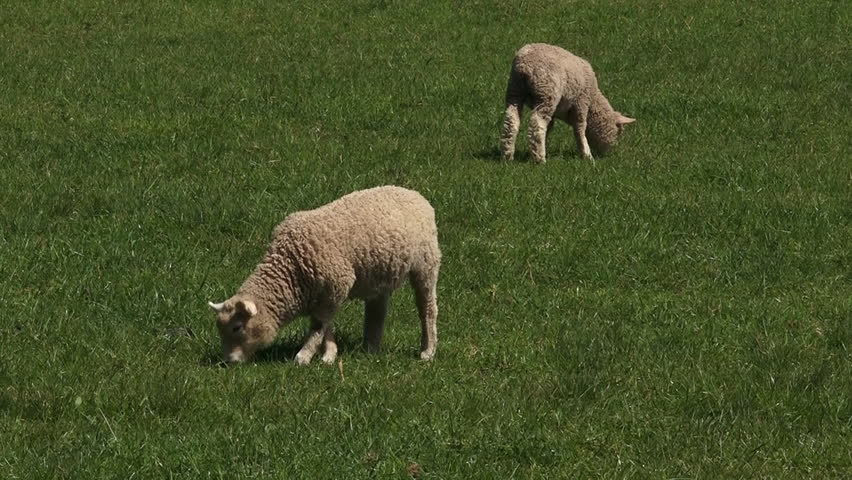
\includegraphics[width=\textwidth]{../Images/input.jpg}
					\caption{Image used in part (a)}
				\end{subfigure}
				\hfill
				\begin{subfigure}[b]{0.47\textwidth}
					\includegraphics[width=\textwidth]{../Output/2_1.jpg}
					\caption{Clustering output (\# Clusters = 8)}
				\end{subfigure}
				\caption{Clustering Original image used in part (a)}
			\end{figure}
		
			\begin{figure}[h]
				\centering
				\begin{subfigure}[b]{0.47\textwidth}
					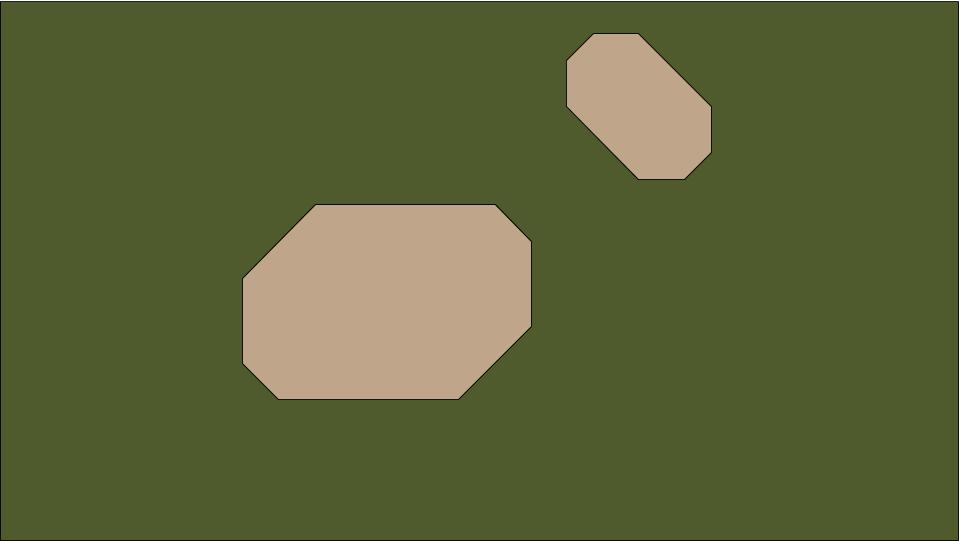
\includegraphics[width=\textwidth]{../Images/input_simple.jpg}
					\caption{Image used in part (a)}
				\end{subfigure}
				\hfill
				\begin{subfigure}[b]{0.47\textwidth}
					\includegraphics[width=\textwidth]{../Output/2_2.jpg}
					\caption{Clustering output (\# Clusters = 5)}
				\end{subfigure}
				\caption{Clustering synthetic image used in part (a)}
			\end{figure}
			
			\item Clustering results with image used in part (b). Parameters used: $\sigma = 2$, $k = 100$, $min = 500$. As we can see from the results in Figure 25 that all the dogs are successfully segmented by the new algorithm. 
			\begin{figure}[!htb]
				\centering
				\begin{subfigure}[b]{0.47\textwidth}
					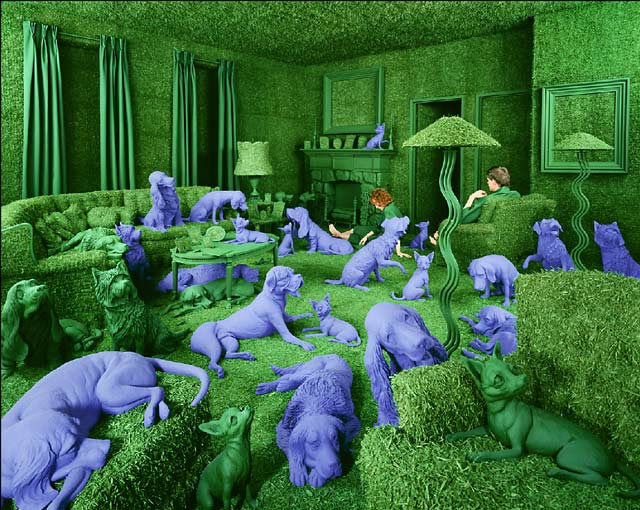
\includegraphics[width=\textwidth]{../Images/green_house.jpg}
					\caption{Image used in part (b)}
				\end{subfigure}
				\hfill
				\begin{subfigure}[b]{0.47\textwidth}
					\includegraphics[width=\textwidth]{../Output/2_3.jpg}
					\caption{Clustering output (\# Clusters = 81)}
				\end{subfigure}
				\caption{Clustering complex image used in part (b)}
			\end{figure}
			
			\newpage
			\item The algorithm is very sensitive to its parameters. I first checked how the algorithm's output varies as we increase the value of $\sigma$. We can clearly see from the results below that the large value of $\sigma$ blurs the boundary between segments and thus makes the algorithm cluster them as a single segment. For the image below, the palm tree got confused with ocean on increasing $\sigma$. 
			
			\begin{figure}[!htb]
				\centering
				\hfill
				\begin{subfigure}[b]{0.30\textwidth}
					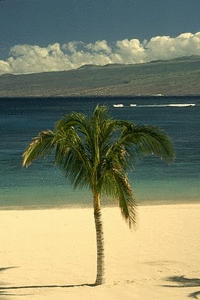
\includegraphics[width=\textwidth]{../Images/beach.jpg}
					\caption{Original Image}
				\end{subfigure}
				\hfill
				\begin{subfigure}[b]{0.30\textwidth}
					\includegraphics[width=\textwidth]{../Output/2_41.jpg}
					\caption{For a decent $\sigma$ value}
				\end{subfigure}
				\hfill
				\begin{subfigure}[b]{0.30\textwidth}
					\includegraphics[width=\textwidth]{../Output/2_42.jpg}
					\caption{For large $\sigma$ value}
				\end{subfigure}
				\caption{Clustering results with change in $\sigma$}
			\end{figure}
		
			\item The results below shows how algorithm behaves as we change the value of the parameter $k$. We can see that as we increase $k$ the clustering becomes more and more aggressive. 
				
				\begin{figure}[!htb]
					\centering
					\begin{subfigure}[b]{0.30\textwidth}
						\includegraphics[width=\textwidth]{../Output/2_41.jpg}
						\caption{For a decent $k$ value}
					\end{subfigure}
					\begin{subfigure}[b]{0.30\textwidth}
						\includegraphics[width=\textwidth]{../Output/2_5.jpg}
						\caption{For large $k$ value}
					\end{subfigure}
					\caption{Clustering results with change in $k$}
				\end{figure}
			
			\item The results below shows how algorithm behaves as we change the value of the parameter $min$. We can see that as we decrease the value of $min$ more smaller clusters start getting identified by the algorithm. 
			
			\begin{figure}[!htb]
				\centering
				\begin{subfigure}[b]{0.45\textwidth}
					\includegraphics[width=\textwidth]{../Output/2_1.jpg}
					\caption{For a decent $min$ value}
				\end{subfigure}
				\begin{subfigure}[b]{0.45\textwidth}
					\includegraphics[width=\textwidth]{../Output/2_6.jpg}
					\caption{For a smaller $min$ value}
				\end{subfigure}
				\caption{Clustering results with change in $min$}
			\end{figure}
		
	\end{enumerate}

	\paragraph{Comparison with N-cut}
	 Compared to N-cut algorithm, `Efficient Graph-Based segmentation' is very very fast. Even for quite high resolution images the segmentation was done within few seconds. On the other hand, N-cut algorithm's space requirement is so huge that it cannot be used for high resolution images. It requests for space in thousands of gigabytes for such images. In terms of performance also the new algorithm is superior to N-cut. It can compute more complex segments as compared to N-cut. 
	
	
	
	\end{homeworkProblem}	
\end{document}